\documentclass[12pt, letterpaper]{article}
\usepackage{graphicx} % Required for inserting images
\usepackage{amsmath}
\usepackage{mdframed}

\title{telegraph equations solved with MFEM library}
\author{Denis Lachapelle}
\date{February 2025}

\setlength{\parindent}{0pt}

\begin{document}

\maketitle

\section{Introduction}
This document explains the telegraph equations simulation using finite differences method based on MFEM library.


\section{Theory, Finite Differences}

The telegraph equations are:

\begin{equation}\frac{\partial{V}}{\partial{x}} + L \frac{\partial{I}}{\partial{t}} + R I = 0\end{equation}


\begin{equation}\frac{\partial{I}}{\partial{x}} + C \frac{\partial{V}}{\partial{t}} + G V = 0\end{equation}


\begin{enumerate}
\item Assume the TL is divided in N segments with node 0 to N. There is N+1 nodes. So nodes are located at $n \Delta x$.
\item Time is sampled at $k \Delta T$.
\item Assume the $\frac{\partial V(t, x)}{\partial x}$ and $\frac{\partial I(t, x)}{\partial x}$ are constant over each segment.
\end{enumerate}

So at a given time $k \Delta T$ we can express the $\frac{\partial V(t, x)}{\partial x}$ and $\frac{\partial I(t, x)}{\partial x}$ as difference  $\frac{V(k \Delta T, (n+1) \Delta x) - V(k \Delta T, (n-1) \Delta x)}{2 \Delta x}$ and  $\frac{I(k \Delta T, (n+1) \Delta x) - I(k \Delta T, (n-1) \Delta x)}{2 \Delta x}$.\\

with the $\frac{\partial}{\partial t}$ on the left side.

\begin{equation} \frac{\partial{I}}{\partial{t}} = - \frac{R I}{L} - \frac{1}{L} \frac{\partial{V}}{\partial{x}} \end{equation}


\begin{equation} \frac{\partial{V}}{\partial{t}} = -\frac{G V}{C} - \frac{1}{C} \frac{\partial{I}}{\partial{x}}\end{equation}




We can write matrix equations....

\begin{equation}
\frac{\partial{I}}{\partial{t}} 
=
	\begin{bmatrix}
		Dv & Ri
	\end{bmatrix}
	\begin{bmatrix}
		V^k \\
		I^k \\
	\end{bmatrix}
\end{equation}

\begin{equation}
	\frac{\partial{V}}{\partial{t}} 
	=
	\begin{bmatrix}
		Gv & Di
	\end{bmatrix}
	\begin{bmatrix}
		V^k \\
		I^k \\
	\end{bmatrix}
\end{equation}

The two equations above can be written as a single matrix equation...

\begin{equation}
    \begin{bmatrix}
    	\frac{\partial{V}}{\partial{t}} \\
    	\frac{\partial{I}}{\partial{t}} 
    \end{bmatrix}	
	=
	\begin{bmatrix}
		Gv Di \\
		Dv Ri
	\end{bmatrix}
	\begin{bmatrix}
		V^k \\
		I^k \\
	\end{bmatrix}
\end{equation}


Where Dv and Di are the same derivative matrix multiplied by different terms -1/L for Dv and -1/C for Di.

\begin{equation}
	\begin{bmatrix}
	   0 & -1/2h & 0 & 0 & ... &0 &0 \\
	   1/2h & 0 &-1/2h & 0 & 0 &... &0 \\
	   0& 1/2h & 0 &-1/2h & 0 &... &0 \\
	   0& 0& 01/2h & 0 &-1/2h & ... &0 \\
	   0& 0& 0&... 1/2h & 0 &-1/2h &0  \\
	   0& 0& 0&... & 1/2h & 0 & 1/2h  \\
	   0& 0& 0& 0&... & 1/2h & 0  \\
	\end{bmatrix}
\end{equation}

Gv and Ri are identity matrix scale by either -G/C and -R/L.

For Dv the multiplier value will be $\frac{\Delta t}{L h}$.\\

Using the above operator we will step in time using RK4.

In principle it produce something like this...


\begin{equation}
	\begin{bmatrix}
		V^{k+1} \\
		I^{k+1} \\
	\end{bmatrix}
	=
	\begin{bmatrix}
		V^k \\
		I^k \\
	\end{bmatrix}
	+
	\Delta t
	\begin{bmatrix}
		\frac{\partial{V}}{\partial{t}} \\
		\frac{\partial{I}}{\partial{t}} 
	\end{bmatrix}	
\end{equation}

\begin{equation}
	\begin{bmatrix}
		V^{k+1} \\
		I^{k+1} \\
	\end{bmatrix}
	=
	\begin{bmatrix}
		V^k \\
		I^k \\
	\end{bmatrix}
	+
	\Delta t
	\begin{bmatrix}
		Gv Di \\
		Dv Ri
	\end{bmatrix}
	\begin{bmatrix}
		V^k \\
		I^k \\
	\end{bmatrix}	
\end{equation}


\subsection{MFEM Implementation}

The program is named stltfdrk4.cpp for Single Transmission Line Transient Finite Difference runge kutta 4.

The signal injected is  gaussian pulse centered at 100ns with a Tau of 20ns multiplied by a triangular window of 200ns wide centered at 100ns.\\

\begin{figure}[h]
	\centering
	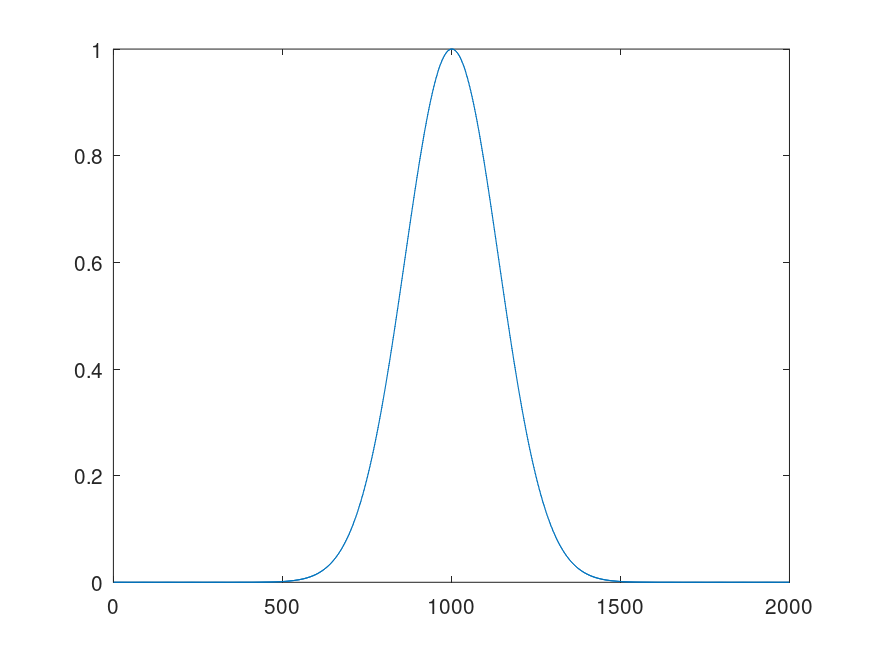
\includegraphics[width=0.8\textwidth]{gaussian_pulse.png} % Adjust width as needed
	\caption{Test pulse}
	\label{fig:example}
\end{figure}

The software do not work fine; I cant find any error. the next step...
\begin{itemize}
	\item rewrite the software in python or octave.
\end{itemize}

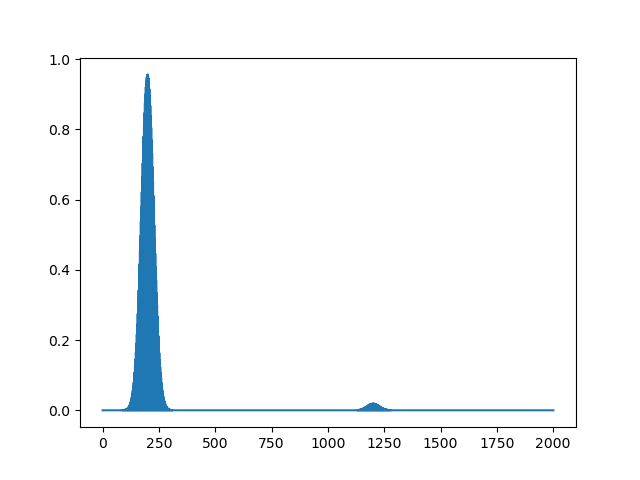
\includegraphics{python-with-zero.png}

ChatGPT:
the resulting signal appear to be with a zero on all odd nodes.
	
	
	ChatGPT said:
	Yes, if the resulting signal shows zeros on all odd nodes (e.g., nodes 1, 3, 5, ...), it's a strong hint that there’s a structural symmetry or a bug in the way your system is discretized — particularly in how the derivative matrices Di and Dv are built.\\
	
The solution according to chatgpt is to have nbrSeg+1 voltage nodes and nbrSeg current in between voltage nodes. So the block matrix will be like this:

\begin{equation}
	\begin{bmatrix}
		\frac{\partial{V}}{\partial{t}} \\
		\frac{\partial{I}}{\partial{t}} 
	\end{bmatrix}	
	=
	\begin{bmatrix}
		Gv Di \\
		Dv Ri
	\end{bmatrix}
	\begin{bmatrix}
		V^k \\
		I^k \\
	\end{bmatrix}
\end{equation}

Gv dimensions will be nbrSeg+1 by nbrSeg+1.\\
Di dimensions will be nbrSeg+1 by nbrSeg.\\
Dv dimensions will be nbrSeg by nbrSeg+1.\\
Ri dimensions will be nbrSeg by nbrSeg.\\

So the block matrix dimensions are 2 nbrSeg+1 by 2 nbrSeg+1.

\begin{equation}
	\begin{bmatrix}
		N+1, N+1 &  N+1, N \\
		N, N+1 & N, N
	\end{bmatrix}
\end{equation}

The following figure shows the pulse propagating along a 100m RG-58 transmission line.

\begin{figure}[h]
	\centering
	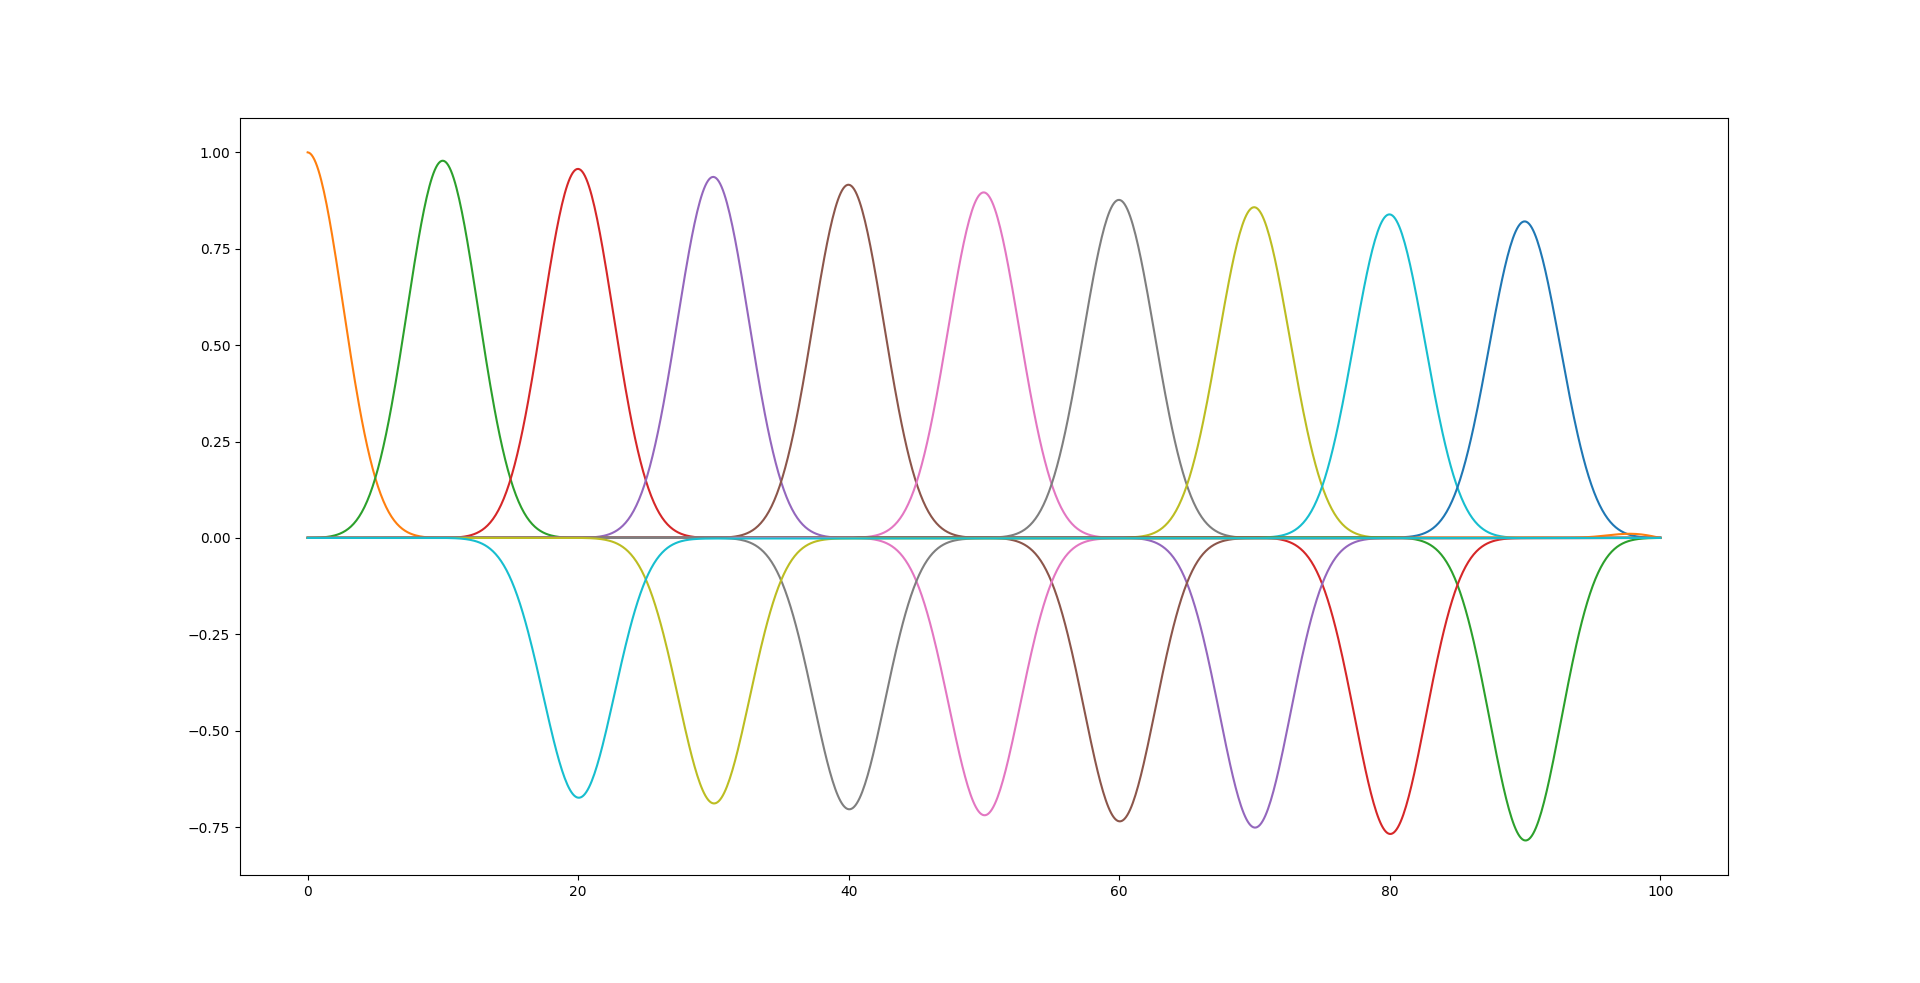
\includegraphics[width=0.8\textwidth]{pulse-python.png} % Adjust width as needed
	\caption{Test pulse propagating}
	\label{fig:example}
\end{figure}

The simulation works fine using Euler Forward difference to differentiate v(x) and I(x) against x and Runge Kutta 4 for time stepping.\\

The reflected voltage is inverted, this looks like the end of the transmission line is shorted, this is the case because the last row is all zero, so di/dx cannot be ... THAT WILL BE TO COMPLETE.\\

To add the source with a serie resistor we should write the equation for $\frac{\partial{V_0}}{\partial{t}}$ which one will repalace the first row equations. The equation is the same as equation 4 with added current from Rs.



\begin{equation} \frac{\partial{V_0}}{\partial{t}} = -\frac{G V_0}{C} - \frac{1}{C} \frac{\partial{I}}{\partial{x}} + \frac{Vs}{Rs C h} - \frac{V_0}{Rs C h}
\end{equation}

The block matrix take care of the transmission line and the following code lines take care of the left and right boundary conditions.

\begin{verbatim}

#apply the left boundary condition which is a voltage source with Rs in séries.
x[0, 0] = x[0, 0] + deltaT*(SourceFunction(Time) - x[0, 0])/(Rs*C*h)

#apply the right boundary condition whichis a load Rl.
x[nbrSeg, 0] = x[nbrSeg, 0] - deltaT*x[nbrSeg, 0]/(Rl*C*h)
\end{verbatim}

But this method makes the RK4 not applied to the boundary. So the best way would be to include the boundary conditions within the block matrix.\\

This done by adding a voltage node Vs, a row to compute Vs.

\begin{itemize}
	\item the first row is to compute Vs which stay the same, so it shall be 1.0 follow by all 0.0.
	\item the second row is 1/(Rs C h) -1/(Rs C h) 0 0 ... 0.
	\item the last sub matrix is all 0.0.
\end{itemize}

The resulting matrix equation is ...


\begin{equation}
	\begin{bmatrix}
		Vs \\
		\frac{\partial{V}}{\partial{t}} \\
		\frac{\partial{I}}{\partial{t}} 
	\end{bmatrix}	
	=
	\left[ 
	\begin{bmatrix}
		0 & 0 & 0 \\
		0 & Gv & Di \\
		0 & Dv & Ri \\
	\end{bmatrix}
	+
		\begin{bmatrix}
		1 & 0 & 0 \\
		\frac{1}{Rs C} & \frac{-1}{Rs C} & 0 \\
		0 & 0 & 0 \\
	\end{bmatrix}
	\right]
	\begin{bmatrix}
		Vs \\
		V^k \\
		I^k \\
	\end{bmatrix}
\end{equation}

Now we need to add the right boundary which is a load Rl. the last voltage node will get influenced by Rl, the equation becomes ...

\begin{equation} \frac{\partial{V_N}}{\partial{t}} = -\frac{G V_N}{C} - \frac{1}{C} \frac{\partial{I}}{\partial{x}} - \frac{V_N}{Rl C h}
\end{equation}

The resulting matrix equation is ...


\begin{equation}
	\begin{bmatrix}
		Vs \\
		\frac{\partial{V}}{\partial{t}} \\
		\frac{\partial{I}}{\partial{t}} 
	\end{bmatrix}	
	=
	\left[ 
	\begin{bmatrix}
		0 & 0 & 0 \\
		0 & Gv & Di \\
		0 & Dv & Ri \\
	\end{bmatrix}
	+
	\begin{bmatrix}
		1 & 0 & 0 \\
		\frac{1}{Rs C h} & \frac{-1}{Rs C h} & 0 \\
		0 & 0 & 0 \\
	\end{bmatrix}
	+
	\begin{bmatrix}
		0 & 0 & 0 \\
		0 & \frac{-1}{Rs C h} & 0 \\
		0 & 0 & 0 \\
	\end{bmatrix}
	\right]
	\begin{bmatrix}
		Vs \\
		V^k \\
		I^k \\
	\end{bmatrix}
\end{equation}


	
\end{document}
